\documentclass{exam}

\usepackage{indentfirst}
\usepackage{graphicx}
\usepackage{listings}
\usepackage{color}
\usepackage{fancyvrb}
\usepackage{url}
\usepackage{amsmath}
\usepackage{algorithm}
\usepackage{algpseudocode}
\usepackage{amsfonts}
\usepackage{amssymb, amsmath, amsthm}
\usepackage{tikz}

\theoremstyle{definition}
\newtheorem{theorem}{Teoremă}
\newtheorem{remark}{Notă}
\newtheorem*{proofsketch}{Demonstrație}

\definecolor{mygreen}{rgb}{0,0.6,0}
\definecolor{mygray}{rgb}{0.5,0.5,0.5}
\definecolor{mymauve}{rgb}{0.58,0,0.82}

\lstset{ %
	backgroundcolor=\color{white},		% choose the background color; you must add \usepackage{color} or \usepackage{xcolor}
	basicstyle=\small\ttfamily,		% the size of the fonts that are used for the code
	breakatwhitespace=false,			% sets if automatic breaks should only happen at whitespace
	breaklines=true,					% sets automatic line breaking
	captionpos=b,						% sets the caption-position to bottom
	columns=fullflexible,
	commentstyle=\color{mygreen},		% comment style
	deletekeywords={...},				% if you want to delete keywords from the given language
	escapeinside={\%*}{*)},			% if you want to add LaTeX within your code
	extendedchars=true,				% lets you use non-ASCII characters; for 8-bits encodings only, does not work with UTF-8
	frame=single,						% adds a frame around the code
	keepspaces=true,					% keeps spaces in text, useful for keeping indentation of code (possibly needs columns=flexible)
	keywordstyle=\color{blue},			% keyword style
	language=Octave,					% the language of the code
	morekeywords={*,...},				% if you want to add more keywords to the set
	%   numbers=left,						% where to put the line-numbers; possible values are (none, left, right)
	%   numbersep=6pt,						% how far the line-numbers are from the code
	%   numberstyle=\tiny\color{mygray},	% the style that is used for the line-numbers
	rulecolor=\color{black},			% if not set, the frame-color may be changed on line-breaks within not-black text (e.g. comments (green here))
	showspaces=false,					% show spaces everywhere adding particular underscores; it overrides 'showstringspaces'
	showstringspaces=false,			% underline spaces within strings only
	showtabs=false,					% show tabs within strings adding particular underscores
	stepnumber=1,						% the step between two line-numbers. If it's 1, each line will be numbered
	stringstyle=\color{mymauve},		% string literal style
	tabsize=2,							% sets default tabsize to 2 spaces
	title=\lstname						% show the filename of files included with \lstinputlisting; also try caption instead of title
}

% Creates a new command to include a perl script, the first parameter is the filename of the script (without .pl), the second parameter is the caption
\newcommand{\octavescript}[2]{
	\lstinputlisting[caption=#2,label=#1]{#1}
}

\newcommand{\MNLab}{Laborator\ \#5}
\newcommand{\MNLabTitle}{Metode iterative pentru rezolvarea sistemelor de ecuații liniare: Jacobi, Gauss-Siedel, Suprarelaxare}
\newcommand{\MNLabTitleHeader}{Metode iterative}
\newcommand{\MNAuthor}{Andrei STAN, Bogdan Țigănoaia}

\renewcommand{\contentsname}{Cuprins}
\renewcommand{\figurename}{Figura}
\newcommand{\norm}[1]{\left\lVert#1\right\rVert}

\setlength{\parskip}{0.5\baselineskip}

\graphicspath{{./img/}}

\title{
	\textmd{\textbf{\MNLabTitle}}
	% \author{Colaboratori: \MNAuthor}
}

\pagestyle{headandfoot}

\header{Metode Numerice}
{\MNLabTitleHeader}
{2025}
\footer{Facultatea de Automatică și Calculatoare}{}{Pagina \thepage\ din \numpages}

\begin{document}

\begin{coverpages}

	\maketitle
	\tableofcontents

\end{coverpages}

\section{Obiective laborator}

\par \^{I}n urma parcurgerii acestui laborator, studentul va fi capabil s\u{a} rezolve sisteme de ecua\c{t}ii liniare utiliz\^{a}nd metode iterative.

\section{Noțiuni teoretice}

\par \textbf{Motivație.} Metodele exacte de rezolvare a sistemelor de ecua\c{t}ii liniare, av\^{a}nd complexitate O(${n}^{3}$), au aplicabilitate limitat\u{a} la ordine de sisteme ce nu dep\u{a}\c{s}esc 1000. Pentru sisteme de dimensiuni mai mari se utilizeaz\u{a} metode cu complexitate O(${n}^{2}$) \^{i}ntr-un singur pas de itera\c{t}ie. Astfel, putem reduce complexitatea totală a algoritmului la O\((\alpha{n}^{2})\), unde \(\alpha\) este o variabila pe care o putem controla, mai precis, numărul de pași utilizați de algoritm. Acestea utilizeaz\u{a} rela\c{t}ii de recuren\c{t}\u{a}, care prin aplicare repetat\u{a} furnizeaz\u{a} aproxima\c{t}ii, cu precizie controlat\u{a}, a solu\c{t}iei sistemului.

\par \textbf{Idee.} Consideram sistemul de $n$ ecuații cu $n$ necunoscute $Ax = b$, unde $A\in\mathbb{R}^{n \times n}$ și $b\in\mathbb{R}^{n}$. Metodele iterative pornesc de la următoarea idee: Av\^{a}nd sistemul $Ax = b$, g\u{a}se\c{s}te o matrice de itera\c{t}ie $G\in\mathbb{R}^{n \times n}$ \c{s}i un vector de itera\c{t}ie $c\in\mathbb{R}^{n}$ astfel \^{i}ncat $x = Gx + c$.  Astfel, pornindu-se cu o aproxima\c{t}ie ini\c{t}ial\u{a} ${x}^{(0)}$ a solu\c{t}iei, rela\c{t}ia de recuren\c{t}\u{a}  folosit\u{a} are format:
\begin{equation} \label{eq:1}
{x}^{(p+1)} = G{x}^{(p)} + c
\end{equation}
unde ${x}^{(p)}, p\in\mathbb{N}$ reprezint\u{a} aproxim\u{a}rea solu\c{t}iei la al $p$-lea pas iterativ.
% \begin{itemize}
% 	\item ${x}^{(0)}, {x}^{(1)}, ... , {x}^{(p)}, ...$ sunt aproxim\u{a}rile solu\c{t}iei;
% 	\item $G$ reprezint\u{a} matricea de itera\c{t}ie;
% 	\item $c$ reprezint\u{a} vectorul de itera\c{t}ie.
% \end{itemize}

% \noindent\makebox[\linewidth]{\rule{\textwidth}{0.4pt}}

\par Prin defini\c{t}ie, o metod\u{a} este \textbf{convergent\u{a}} dac\u{a} \c{s}i numai dac\u{a} 
\begin{equation}\label{eq:convergenta}
\lim_{p\rightarrow \infty}x^{(p)}=\Tilde{x}
\end{equation}
unde $\Tilde{x}$ este solu\c{t}ia unic\u{a} a sistemului $Ax=b$ \c{s}i a sistemului $x=Gx+c$, fiind echivalente.  O astfel de metod\u{a} iterativă este convergent\u{a} dac\u{a} este stabil\u{a} \c{s}i consistent\u{a}.

\noindent\makebox[\linewidth]{\rule{\textwidth}{0.4pt}}
\par \textbf{Teoremă.} Condi\c{t}ia necesar\u{a} \c{s}i suficient\u{a} de convergen\c{t}\u{a} a metodei descrise de ecua\c{t}ia \ref{eq:1} este
$${\rho}(G) < 1$$
unde ${\rho}(G)$ este raza spectrala a matricei $G$.


\par \textbf{Notă.} Prin definiție, ${\rho}(G) = \max(|{\lambda}_{1}|, |{\lambda}_{2}|, ... , |{\lambda}_{k}|)$, unde ${\lambda}_{i}, i = \overline{1,k}$ reprezint\u{a} valorile proprii ale matricei.
\par \textbf{Demonstrație condi\c{t}ie necesar\u{a}.} Considerăm vectorul de eroare la pasul $n$ ca fiind $e^{(p)}=x^{(p)}-\Tilde{x}$. Evident c\u{a}, ecua\c{t}ia \ref{eq:convergenta} este echivalent\u{a} cu $$\lim_{p\rightarrow \infty}e^{(p)}=0$$ unde $0$ denot\u{a} vectorul nul din $\mathbb{R}^n$. Pornind de la ecua\c{t}ia \ref{eq:1}, putem spune c\u{a} 
$${x}^{(p+1)} -\Tilde{x} = G{x}^{(p)} + c -\Tilde{x}$$
\c{s}i pentru că $\Tilde{x}=G\Tilde{x} + c$, avem 
$${x}^{(p+1)} -\Tilde{x} = G{x}^{(p)} - G\Tilde{x} \iff {x}^{(p+1)} -\Tilde{x} = G({x}^{(p)} - \Tilde{x}) \iff e^{(p+1)}=Ge^{(p)}$$

Prin induc\c{t}ie, se demonstreaz\u{a} u\c{s}or c\u{a} $e^{(p+1)}=G^{p+1}e^{(0)}$. Rezult\u{a} astfel c\u{a} metoda este convergent\u{a} dac\u{a} \c{s}i numai dac\u{a} 
\begin{equation} \label{eq:errvect}
\lim_{p\rightarrow \infty}G^{p+1}e^{(0)}=0
\end{equation}

\^{I}n continuare ne propunem s\u{a} demonstr\u{a}m c\u{a} rela\c{t}ia anterioar\u{a} se men\c{t}ine adev\u{a}rat\u{a} dac\u{a} \c{s}i numai dac\u{a} $\rho(G) < 1$. Consider\u{a}m $\norm{\cdot}$ ca fiind norma vectorial\u{a}, respectiv matricial\u{a} peste $\mathbb{R}^n$, respectiv $\mathbb{R}^{n\times n}$.
% Avem astfel, $$\norm{G^{p+1}u} \leq \norm{G^{p+1}} \norm{u}, \forall u \in \mathbb{R}^n$$ 
% Astfel, ecua\c{t}ia \ref{eq:errvect} se \^{i}ndepline\c{s}te doar dac\u{a} $\lim_{p\rightarrow \infty}\norm{G^{p+1}} = 0$.

Presupunem prin reducere la absurd c\u{a} $\rho(G) \geq 1$. \^{I}n special, alegem $e^{(0)}$ vector propriu al matricei $G$, asociat unei valori proprii $\lambda=\rho(G)$ astfel \^{i}nc\^{a}t 
$$G^{p+1}e^{(0)} = \|\lambda\|^{p+1} e^{(0)}$$ 
Trec\^{a}nd la limit\u{a} membrul drept \c{s}i av\^{a}nd \^{i}n vedere c\u{a} $e^{(0)}$ este nenul, ob\c{t}inem c\u{a} 
$$\lim_{p\rightarrow \infty}G^{p+1}e^{(0)} = \lim_{p\rightarrow \infty}\|\lambda\|^{p+1} e^{(0)} \neq 0$$ ceea ce este fals. Astfel, am demonstrat c\u{a} este necesar ca $\rho(G) < 1$.

\textbf{Demonstra\c{t}ia condi\c{t}iei suficiente} se bazeaza pe inegalitatea lui Gelfand pentru raz\u{a} spectral\u{a}. Această demonstrație pentru condiția suficientă este peste scopul laboratorului. Însă, o astfel de demonstrație, formalizată riguros matematic, este prezentată în \cite{Hansen}.

\noindent\makebox[\linewidth]{\rule{\textwidth}{0.4pt}}
% \noindent\makebox[\linewidth]{\rule{\textwidth}{0.4pt}}

% \begin{theorem}
% \par O astfel de metod\u{a} iterativă este convergent\u{a} dac\u{a} este stabil\u{a} \c{s}i consistent\u{a}. 
% Condi\c{t}ia necesar\u{a} \c{s}i suficient\u{a} de convergen\c{t}\u{a} este
% \[
% \rho(G) < 1
% \]
% unde $\rho(G)$ este raza spectral\u{a} a matricei $G$.
% \end{theorem}

% \begin{remark}
% Prin definiție, $\rho(G) = \max(|\lambda_{1}|, |\lambda_{2}|, \dots , |\lambda_{n}|)$, 
% unde $\lambda_{i}, i = \overline{1,n}$ reprezint\u{a} valorile proprii ale matricei.
% \end{remark}

% \begin{proofsketch}
% O demonstrație pentru teorema anterioară este mult peste scopul laboratorului. 
% O astfel de demonstrație formalizată riguros matematic, este prezentată în \cite{Hansen}.
% \end{proofsketch}

\vspace{10pt}

\par \textbf{Descompunerea matricei \(A\)}
\par  Metodele iterative se bazeaz\u{a} pe descompunerea matricei $A$ sub forma $A = N - P$. Atunci sistemul devine: $$Ax=b \iff (N - P)x = b, \iff Nx = Px + b\iff x = {N}^{-1}Px + {N}^{-1}b .$$

Astfel, rezult\u{a} rela\c{t}ia de recuren\c{t}\u{a}:
\begin{equation} \label{eq:2}
{x}^{(p+1)} = {N}^{-1}P{x}^{(p)} + {N}^{-1}b
\end{equation}
de unde putem identifica $G = {N}^{-1}P$ \c{s}i $c = {N}^{-1}b$.

\par În mod convenabil, se parti\c{t}ioneaz\u{a} matricea $A$ pun\^{a}nd \^{i}n eviden\c{t}\u{a} o matrice diagonal\u{a} $D$, o matrice strict triunghiular inferioar\u{a} $L$ \c{s}i o matrice strict triunghiular superioar\u{a} $U$:
$$A = D - L - U.$$

\begin{center}
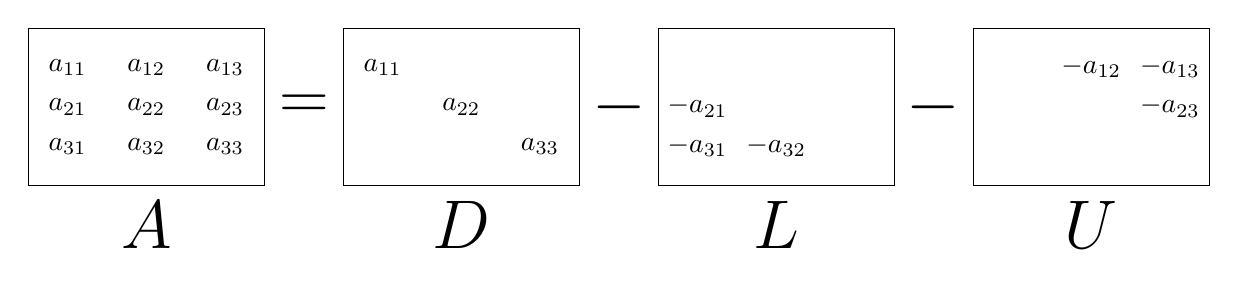
\begin{tikzpicture}
    % Matrix A
    \draw (-2,1) -- (1,1) -- (1,-1) -- (-2,-1) -- cycle;
    \node at (-1.5, 0.5) {$a_{11}$};
    \node at (-0.5, 0.5) {$a_{12}$};
    \node at (0.5, 0.5) {$a_{13}$};
    \node at (-1.5, 0) {$a_{21}$};
    \node at (-0.5, 0) {$a_{22}$};
    \node at (0.5, 0) {$a_{23}$};
    \node at (-1.5, -0.5) {$a_{31}$};
    \node at (-0.5, -0.5) {$a_{32}$};
    \node at (0.5, -0.5) {$a_{33}$};
    \node at (-0.5, -1.5) {\Huge $A$};
    

    % Arrow to decomposition
    % \draw[thick, ->] (1.5,0) -- (2.5,0);
    \node at (1.5, 0) {\Huge $=$};

    % D matrix
    \draw (2,1) -- (5,1) -- (5,-1) -- (2,-1) -- cycle;
    \node at (2.5, 0.5) {$a_{11}$};
    \node at (3.5, 0) {$a_{22}$};
    \node at (4.5, -0.5) {$a_{33}$};
    \node at (3.5, -1.5) {\Huge $D$};
    
    % L matrix
    \node at (5.5,0) {\Huge $-$};
    \draw (6,1) -- (9,1) -- (9,-1) -- (6,-1) -- cycle;
    \node at (6.5, 0) {$-a_{21}$};
    \node at (6.5, -0.5) {$-a_{31}$};
    \node at (7.5, -0.5) {$-a_{32}$};
    \node at (7.5, -1.5) {\Huge $L$};

    % U matrix
    \node at (9.5,0) {\Huge $-$};
    \draw (10,1) -- (13,1) -- (13,-1) -- (10,-1) -- cycle;
    \node at (11.5, 0.5) {$-a_{12}$};
    \node at (12.5, 0.5) {$-a_{13}$};
    \node at (12.5, 0) {$-a_{23}$};
    \node at (11.5, -1.5) {\Huge $U$};
\end{tikzpicture}
\end{center}

\par Diferența dintre cele trei metode studiate în continuare este dată de modul în care se face asocierea convenabil între $D, L, U$ și $N, P$.

\textbf{Rata de convergență și condiția de oprire}

\par Având în vedere condiția de convergență menționata anterior, astfel de metode iterative garantează că la fiecare pas se aproprie mai mult de soluția analitică. Însă, pentru a determina cât de repede sau cât de încet se aproprie de soluție este necesară introducerea conceptului de \textbf{rată de convergență} \cite{Gallier}. Studiul acestui concept este de natură matematică și nu face obiectul acestui laborator. 

\par Pentru a finaliza execuția metodelor iterative din cadrul acestui laborator vom introduce doua condiții: \textbf{toleranța} (notată in continuare cu \(\epsilon\)) și \textbf{numărul maxim de iterații} (notat în continuare cu \(N_{iter}\)). Toleranța ne asigură faptul ca algoritmul nu efectuează iterații mai mult decât este necesar, practic nu se continuă execuția dacă "diferența" soluțiilor a două iterații consecutive nu este semnificativă. Numărul maxim de pași garantează că algoritmul se încheie, indiferent dacă alegerea inițială pentru \(x^{(0)}\) a fost una fructuoasă care în urma algoritmului a rezultat o aproximare numerica bună sau nu.

 % \pagebreak

\subsection{Metoda Jacobi}
\par \^{I}n metoda Jacobi se aleg:
\begin{align*}
N &= D \\
P &= L + U \\
{G}_{J} &= {D}^{-1}(L + U) \\
\end{align*}

\par \textbf{Observație.} Pentru ca matricea $N$ să fie inversabilă, diagonala matricei $A$ trebuie să aibă elementele nenule.

\par Lucrând analitic sistemul \ref{eq:2}, rezulta solu\c{t}ia sistemului:
$${x}_{i}^{(p+1)} = \frac{{b}_{i} - \sum_{j = 1, j \neq i}^{n}{a}_{ij}{x}_{j}^{(p)}}{{a}_{ii}}, i\in\overline{1, n}$$

%\par Metoda converge dac\u{a} matricea $A$ este diagonal dominant\u{a}\footnote{\url{http://en.wikipedia.org/wiki/Diagonally\_dominant\_matrix}}  pe linii ($|{a}_{ii}| > \sum_{j \neq i}|{a}_{ij}| )$.

\begin{algorithm}[H]
\caption{Metoda Iterativă Jacobi în formă nematricială, cu vectorizări}
\label{alg:jacobi}
\begin{algorithmic}[1]
    \State \textbf{Intrare:} Matricea \( A \in \mathbb{R}^{n \times n} \), vectorul \( b \in \mathbb{R}^{n} \), aproximarea inițială \( x^{(0)} \), toleranța \( \epsilon \), numărul maxim de iterații \( N_{iter} \).
    \State  \( x \leftarrow x^{(0)} \) \Comment{Inițializare}
    \For{\( p = 1 \) to \( N_{iter} \)}
        \State \(x_{prev} \gets x\)
        \For{\( i = 1 \) to \( n \)}
            \State \(x(i) \gets b(i) - A(i,1:n) \cdot x_{prev} + A(i,i) \times x_{prev}[i] \) \Comment{Calculul formulei cu vectorizare}
            \State \(x(i) \gets \frac{1}{A(i,i)} \times x(i) \)
            
        \EndFor
        \State
        \If{\( \| x - x_{prev} \| < \epsilon \)} \Comment{Verificarea toleranței}
            \State \textbf{return} \( x \)
        \EndIf
    \EndFor
    \State \textbf{returnează} \( x \)
\end{algorithmic}
\end{algorithm}






\subsection{Metoda Gauss-Seidel}
\par În cadrul metodei Gauss-Seidel, alegerile sunt urmatoarele:
\begin{align*}
N &= D - L \\
P &= U \\
{G}_{GS} &= {(D - L)}^{-1}U
\end{align*}
% $N = D - L$

% $P = U$

% ${G}_{GS} = {(D - L)}^{-1}U$

% \par \textbf{Observație.} 

Solu\c{t}ia analitică sistemului \ref{eq:2} este:
$${x}_{i}^{(p+1)} = \frac{{b}_{i} - \sum_{j = 1}^{i-1}{a}_{ij}{x}_{j}^{(p+1)} - \sum_{j = i + 1}^{n}{a}_{ij}{x}_{j}^{(p)}}{{a}_{ii}}, i\in\overline{1, n}$$

%\par Metoda converge dac\u{a} matricea A este simetric\u{a} (${a}_{ij} = {a}_{ji},  i,j = 1:n$) \c{s}i pozitiv definit\u{a} ($\forall z \in R^{n}, {z}^{T}Az >0$).


\vspace{100pt}
\par \textbf{Observa\c{t}ii:}
\begin{enumerate}
        \item  Pentru ca matricea $N$ să fie inversabilă, determinantul acesteia trebuie sa fie nenul. Deoarece determinantul unei matrice triunghiulară este produsul elementelor de pe diagonală, înseamnă ca acestea trebuie să fie nenule.
	\item  Dac\u{a} matricea sistemului este diagonal dominant\u{a} pe linii, metoda Gauss Seidel este convergent\u{a}. Reciproca nu este adevarat\u{a}.
	\item  O matrice $A$ este diagonal dominant\u{a} pe linii dac\u{a} \c{s}i numai dac\u{a} are urm\u{a}toarea proprietate: pentru fiecare linie i, modulul elementului de pe diagonala principal\u{a}, $A(i,i)$ este strict mai mare dec\^{a}t suma modulelor elementelor de pe aceea\c{s}i linie $i$.
\end{enumerate}

\begin{algorithm}[H]
\caption{Metoda Iterativă Gauss-Seidel în formă nematricială, cu vectorizări}
\label{alg:gauss_seidel}
\begin{algorithmic}[1]
    \State \textbf{Intrare:} Matricea \( A \in \mathbb{R}^{n \times n} \), vectorul \( b \in \mathbb{R}^{n} \), aproximarea inițială \( x^{(0)} \), toleranța \( \epsilon \), numărul maxim de iterații \( N_{iter} \).
    \State \( x \leftarrow x^{(0)} \)  \Comment{Inițializare}
    \For{\( p = 1 \) to \( N_{iter} \)}
        \State \(x_{prev} \gets x \)
        \For{\( i = 1 \) to \( n \)}
            \State \( S_1 \gets A(i,1:i-1)\cdot x(1:i-1) \) \Comment{Folosim valori calculate la pasul curent}
            \State \( S_2 \gets A(i,i+1:n) \cdot x_{prev}(i+1:n) \) \Comment{Folosim valori de la pasul anterior}
            \State \( x^{(p)}[i] \gets \frac{b[i] - S_1 - S_2}{A[i,i]} \) \Comment{Actualizare}
        \EndFor
        \If{\( \| x - x_{prev} \| < \epsilon \)} 
            \State \textbf{return} \( x \)
        \EndIf
    \EndFor
    \State \textbf{returnează} \( x \)
\end{algorithmic}
\end{algorithm}


\subsection{Metoda suprarelax\u{a}rii}
Pentru g\u{a}sirea unei descompuneri c\^{a}t mai rapid convergente, se introduce parametrul de relaxare $\omega$:
$$A = N - P = N - \omega N - P + \omega N = (1 - \omega)N - (P - \omega N) = N(\omega) - P(\omega)$$

de unde ob\c{t}inem:
\begin{align*}
N(\omega) &= (1 - \omega)N \\
P(\omega) &= P - \omega N \\
G(\omega) &= {N}^{-1}(\omega)P(\omega)\\ &= \frac{{N}^{-1}}{1-\omega}(P - \omega N)\\ &= \frac{{N}^{-1}P - \omega{I}_{n}}{1-\omega} 
\end{align*}



Condi\c{t}ia de stabilitate impune $\omega \in (0,2)$. \^{I}n practic\u{a} se face o alt\u{a} alegere, astfel:

$N(\omega) = \frac{1}{\omega}D - L, \quad P(\omega) = (\frac{1}{\omega} - 1)D + U, \quad {G}_{\omega} = (D-\omega L)^{-1}[(1-\omega)D+\omega U]$

Solu\c{t}ia sistemului se poate scrie sub forma:
$$x_{i}^{(p+1)}=\omega\frac{{b}_{i} - \sum_{j = 1}^{i-1}{a}_{ij}{x}_{j}^{(p+1)} - \sum_{j = i + 1}^{n}{a}_{ij}{x}_{j}^{(p)}}{{a}_{ii}}+(1-\omega)x_{i}^{(p)}$$

Dac\u{a} se alege $\omega = 1 \Rightarrow$ metoda Gauss-Seidel.

\begin{algorithm}[H]
\caption{Metoda Iterativă Gauss-Seidel cu Suprarelaxare (SOR)}
\label{alg:sor}
\begin{algorithmic}[1]
    \State \textbf{Intrare:} Matricea \( A \in \mathbb{R}^{n \times n} \), vectorul \( b \in \mathbb{R}^{n} \), aproximarea inițială \( x^{(0)} \), factorul de relaxare \( \omega \), toleranța \( \epsilon \), numărul maxim de iterații \( N_{iter} \).
    \State \textbf{Inițializare:} \( x \leftarrow x^{(0)} \)
    \For{\( p = 1 \) to \( N_{iter} \)}
        \State \( x_{\text{prev}} \gets x \) \Comment{Salvăm valorile anterioare}
        \For{\( i = 1 \) to \( n \)}
            \State \( S_1 \gets A(i,1:i-1) \cdot x(1:i-1) \) \Comment{Valori noi}
            \State \( S_2 \gets A(i,i+1:n) \cdot x_{\text{prev}}(i+1:n) \) \Comment{Valori vechi}
            \State \( x^{(p)}[i] \gets \frac{b[i] - S_1 - S_2}{A[i,i]} \) \Comment{Gauss-Seidel}
            \State \( x[i] \gets \omega \cdot x^{(p)}[i] + (1 - \omega) \cdot x_{\text{prev}}[i] \) \Comment{Suprarelaxare}
        \EndFor
        \If{\( \| x - x_{\text{prev}} \| < \epsilon \)}
            \State \textbf{return} \( x \)
        \EndIf
    \EndFor
    \State \textbf{returnează} \( x \)
\end{algorithmic}
\end{algorithm}


\section{Probleme rezolvate}

\subsection{Problema 1}

S\u{a} se rezolve sistemul folosind metoda Gauss-Seidel:
$$	\left\{
	\begin{array}{ccccccc}
		7x_1 & + & 2x_2 & - & 4x_3 & = & 7  \\
		3x_1 & + & 6x_2 & + & 2x_3 & = & 15 \\
		2x_1 & - & 5x_2 & + & 8x_3 & = & 28 \\
	\end{array} \right.
$$

\textit{Solu\c{t}ie}:

Scriem formulele de recuren\c{t}\u{a}

$$\left\{
	\begin{array}{ccccccccc}
		x_1^{(k+1)} & = & -2/7x_2^{(k)} & + & 4/7x_3^{(k)} & + & 7/7  \\
		x_2^{(k+1)} & = & -3/6x_1^{(k)} & - & 2/6x_3^{(k)} & + & 15/6 \\
		x_3^{(k+1)} & = & -2/8x_1^{(k)} & + & 5/8x_2^{(k)} & + & 28/8 \\
	\end{array} \right.
$$

Dac\u{a} alegem $x_{1}^{(0)} = x_{2}^{(0)}=x_{3}^{(0)}=0$ ob\c{t}inem urm\u{a}toarele rezultate:
$$  \begin{array}{c||ccc}
		k & x_1^{(k)} & x_2^{(k)} & x_3^{(k)} \\
		\hline
		0 & 0         & 0         & 0         \\
		1 & 1         & 2         & 4.5       \\
		2 & 3.00      & -0.5      & 2.43      \\
		3 & 2.53      & 0.41      & 3.12      \\
		4 & 2.66      & 0.12      & 2.91      \\
		5 & 2.62      & 0.21      & 2.97      \\
	\end{array}
$$

Solu\c{t}ia exact\u{a} este: $x_{1}=2.63,\ x_{2}=0.19\ x_{3}=2.96$.
%\end{Problem}

\subsection{Problema 2}
Folosi\c{t}i metoda Jacobi pentru a aproxima solu\c{t}ia sistemului:
$$	\left\{
	\begin{array}{ccccccc}
		10x_1 & - & 5x_2  & + & x_3   & = & 1 \\
		x_1   & + & 4x_2  & + & 3 x_3 & = & 4 \\
		4x_1  & - & 3 x_2 & - & 9x_3  & = & 6 \\
	\end{array} \right.
$$

\textit{Solu\c{t}ie}:

Scriem formulele de recuren\c{t}\u{a}
$$\left\{
	\begin{array}{ccccccc}
		x_1^{(k+1)} & = & 5/10x_2^{(k)} & - & 1/10x_3^{(k)} & + & 1/10 \\
		x_2^{(k+1)} & = & -1/4x_1^{(k)} & - & 3/4x_3^{(k)}  & + & 4/4  \\
		x_3^{(k+1)} & = & 4/9x_1^{(k)}  & - & 3/9x_2^{(k)}  & - & 6/9  \\
	\end{array} \right.
$$

Aleg\^{a}nd $x_{1}^{(0)}=x_{2}^{(0)}=x_3^{(0)}=0\Rightarrow$


$$  \begin{array}{c||ccc}
		k & x_1^{(k)} & x_2^{(k)} & x_3^{(k)} \\
		\hline
		0 & 0         & 0         & 0         \\
		1 & 0.1       & 1.00      & -0.66     \\
		2 & 0.66      & 1.47      & -1.95     \\
		3 & 0.93      & 1.55      & -0.86     \\
		4 & 0.96      & 1.41      & -0.76     \\
		5 & 0.88      & 1.33      & -0.71     \\
	\end{array}
$$

Solu\c{t}ia exact\u{a} este: $x_{1}=0.84,\ x_{2}=1.34,\ x_{3}=-0.73$.
%\end{Problem}

\subsection{Problema 3}
Fie sistemul $Ax=b, A \in R^{2\times 2}, x, b \in R^{2},
	A =
	\left[ {\begin{array}{cc}
					2 & 2 \\
					1 & 3
				\end{array} } \right]
$. Matricea $A$ nu este diagonal dominant\u{a} pe linii. \^{I}n aceste condi\c{t}ii este convergent\u{a} metoda Gauss-Seidel?

\textit{Solu\c{t}ie}:

Se determin\u{a} matricea de itera\c{t}ie a sistemului pentru metoda Gauss-Seidel, ${G}_{GS}$.

$A = D - L - U \Rightarrow \quad D = \left[ {\begin{array}{cc}
					2 & 0 \\
					0 & 3
				\end{array} } \right], \quad L =
	\left[ {\begin{array}{cc}
					0  & 0 \\
					-1 & 0
				\end{array} } \right], \quad U =
	\left[ {\begin{array}{cc}
					0 & -2 \\
					0 & 0
				\end{array} } \right]$

Atunci:

${G}_{GS} = {(D-L)}^{-1}U =
	\left[ {\begin{array}{cc}
					2 & 0 \\
					1 & 3
				\end{array} } \right] ^ {-1}
	\left[ {\begin{array}{cc}
					0 & -2 \\
					0 & 0
				\end{array} } \right]
	=
	\left[ {\begin{array}{cc}
					0 & -1          \\
					0 & \frac{1}{3}
				\end{array} } \right]$.

$\det{(\lambda I - G_{GS})} = \left| {\begin{array}{cc}
		\lambda & 1                     \\
		0       & \lambda - \frac{1}{3}
	\end{array} } \right| = 0\Rightarrow \lambda(G_{GS}) = \{0,\frac{1}{3}\}$  \c{s}i $\rho(G_{GS}) = \frac{1}{3} < 1$.

$\Rightarrow$ metoda Gauss-Seidel este convergent\u{a}.
%\end{Problem}


\subsection{Problema 4}
S\u{a} se implementeze o func\c{t}ie OCTAVE care rezolv\u{a} un sistem de ecua\c{t}ii liniare folosind metoda iterativ\u{a} Gauss-Seidel. Date de intrare: $A$ - matricea sistemului; $b$ - vectorul termenilor liberi; $x0$ - aproxima\c{t}ia ini\c{t}ial\u{a} a solu\c{t}iei; $tol$ - precizia determin\u{a}rii solu\c{t}iei; $maxiter$ - num\u{a}rul maxim de itera\c{t}ii. Date de ie\c{s}ire: $x$ - solu\c{t}ia sistemului; $succes$ - variabilă care indică convergenţa metodei.

\textit{Solu\c{t}ie}:

\octavescript{./src/GaussSeidel.m}{}

\begin{center}
	\begin{tabular}{| l | l |}
		\hline
		\textbf{Date de intrare:}  & \textbf{Date de ieşire:} \\
		$A = $
		$\left[ {\begin{array}{cc}
							         2 & 2 \\
							         1 & 3
						         \end{array} } \right],$

		$b = $
		$\left[ {\begin{array}{cc}
							         2 \\
							         1
						         \end{array} } \right],$

		$x0 =
			\left[ {\begin{array}{cc}
							        0 \\
							        0
						        \end{array} } \right],$

		$ tol=0.0001, maxiter=100$ &
		$x = $
		$\left[ {\begin{array}{cc}
							         1 \\
							         0
						         \end{array} } \right]$
		\\
		\hline
	\end{tabular}
\end{center}
%\end{Problem}

\section{Probleme propuse}

%--------------------------------------------------------------------------------------
%	PROBLEM 1
%--------------------------------------------------------------------------------------
\subsection{Problema 1}
Fie sistemul $Ax=b, A \in R^{2 \times 2}, b \in R^{2}$, cu
$A =\left[ {\begin{array}{cc}
					2  & -1 \\
					-1 & 2
				\end{array} } \right]$. Determina\c{t}i raza spectral\u{a} a matricei de itera\c{t}ie Jacobi. Stabili\c{t}i convergen\c{t}a metodei Jacobi.
%\end{Problem}

%----------------------------------------------------------------------------------------
%       PROBLEM 2
%----------------------------------------------------------------------------------------

% To have just one problem per page, simply put a \clearpage after each problem

\subsection{Problema 2}
Fie sistemul liniar:
$$	\left\{
	\begin{array}{ccccccc}
		2x & + & y  & + & z  & = & 4 \\
		x  & + & 2y & + & z  & = & 4 \\
		x  & + & y  & + & 2z & = & 4 \\
	\end{array} \right.
$$

Stabili\c{t}i:
%\begin{enumerate}

a) dac\u{a} matricea sistemului este diagonal dominant\u{a} pe linii;

b) convergen\c{t}a metodei Jacobi;

c) convergen\c{t}a metodei Gauss-Seidel.
%\end{enumerate}

\^{I}n caz de convergen\c{t}\u{a}, calcula\c{t}i solu\c{t}ia iterativ\u{a} dup\u{a} trei pa\c{s}i. Alege\c{t}i voi aproxima\c{t}ia ini\c{t}ial\u{a}.

%\end{Problem}

%----------------------------------------------------------------------------------------
%       PROBLEM 3
%----------------------------------------------------------------------------------------
\subsection{Problema 3}
Fie o matrice $A \in R^{n\times n}$ tridiagonal\u{a} \footnote{\url{http://mathworld.wolfram.com/TridiagonalMatrix.html}} \c{s}i sistemul de ecua\c{t}ii $Ax=b$, cu $b,\ x \in R^{n}$. Scrie\c{t}i o func\c{t}ie OCTAVE care rezolv\u{a} sistemul de ecua\c{t}ii prin metoda iterativ\u{a} Jacobi.

\octavescript{./src/Jacobi.m}{Algoritmul Jacobi}
%\end{Problem}

%-----------------------------------------------------------------------------------------
%       PROBLEM 4
%-----------------------------------------------------------------------------------------
\subsection{Problema 4}
S\u{a} se implementeze o func\c{t}ie OCTAVE care rezolv\u{a} un sistem liniar de ecua\c{t}ii folosind metoda suprarelax\u{a}rii.
\octavescript{./src/sor.m}{Suprarelaxare}

S\u{a} se testeze func\c{t}ia folosind diferite valori pentru $\omega$.
%\end{Problem}     

\bibliographystyle{ieeetr}
\bibliography{refs}

\end{document}
